%%%%%%%%%%%%%%%%%%%%%%%%%%%%%%
% Ioannis Petrousov
% petrousov@gmail.com
% 2025
%
% Custom Latex thesis template
% to be used for English language.
%
% Initial compile:
%     1. xelatex
%     2. bibtex
%     3. xelatex
%     4. xelatex
%
% Further compile:
%
% A: If you change the bibliography file
%     1. biblatex
%     2. xelatex
%     3. xelatex
%
% B: If you DONT change the bibliography file
%     1. xelatex
%     2. xelatex
%%%%%%%%%%%%%%%%%%%%%%%%%%%%%%

% Use the following documentclass declaration if you plan to make a hardcopy
% The twoside option shift text for making a book print
%\documentclass[12pt,twoside]{report}

% Use the following documentclass for PDF and to view on computer only
\documentclass[8pt,a4paper]{report}%{book}

\usepackage{listings}
\usepackage{csquotes}

\usepackage{float}
% TEXT FORMATTING
% set spacing between lines (line spacing)
\usepackage{setspace}
\setstretch{1.5}
% package to customize chapters, sections and subsections style
\usepackage{titlesec}
% chapter title appearance format
\titleformat{\chapter}[display]
{\bfseries\huge}{\chaptertitlename\space}{16pt}{}
% https://www.sharelatex.com/learn/Sections_and_chapters
\titlespacing{\chapter}{0pc}{1.5ex plus .1ex minus .2ex}{5pc}
% section title appearance format
\titleformat{\section}
{\bfseries\large}{\thesection}{14pt}{}
% subsection title appearance format
\titleformat{\subsection}
{\bfseries\normalsize}{\thesubsection}{12pt}{}
% set margins
\usepackage{geometry}
\geometry{left=3cm, right=2cm, top=2.5cm, bottom=2.5cm}
% text justification is fully-justified by default

% xelatex wants fontspec
\usepackage{fontspec}
\usepackage{xltxtra}
% \setmainfont[Mapping=tex-text]{Latin Modern Roman}
\setmainfont[Mapping=tex-text]{XITS}
% package allows to place figures
\usepackage{graphicx}
% put images in images path
\graphicspath{{images/}}
\usepackage{setspace}

% Caption customization
% use this package to set appearance for captions
\usepackage{caption}
% caption size for figures 10pt
\captionsetup[figure]{font=footnotesize,labelfont=footnotesize}
% caption size for tables 10pt and underlined
\usepackage[normalem]{ulem} % Package for underlining
\DeclareCaptionLabelFormat{label_format}{\uline{#1~#2}} % underline label
\DeclareCaptionTextFormat{text_format}{\uline{#1}} % underline text
\DeclareCaptionLabelSeparator{separator_format}{\uline{:~}} % underline separator
%\captionsetup[table]{font=normalsize,labelfont=normalsize,labelformat=label_format,textformat=text_format,labelseparator=separator_format}

% use this package to define custom colors
\usepackage{xcolor}

% create colors
\colorlet{punct}{red!60!black}
\definecolor{background}{HTML}{EEEEEE}
\definecolor{delim}{RGB}{20,105,176}
\colorlet{numb}{magenta!60!black}

% listing colors
\definecolor{codegreen}{rgb}{0,0.6,0}
\definecolor{codegray}{rgb}{0.5,0.5,0.5}
\definecolor{codepurple}{rgb}{0.58,0,0.82}
\definecolor{backcolour}{rgb}{0.95,0.95,0.92}

\lstdefinestyle{mystyle}{
    backgroundcolor=\color{backcolour},
    commentstyle=\color{codegreen},
    keywordstyle=\color{magenta},
    numberstyle=\tiny\color{codegray},
    stringstyle=\color{codepurple},
    basicstyle=\ttfamily\footnotesize,
    breakatwhitespace=false,
    breaklines=true,
    captionpos=b,
    keepspaces=true,
    numbers=left,
    numbersep=5pt,
    showspaces=false,
    showstringspaces=false,
    showtabs=false,
    tabsize=2
}

\lstset{style=mystyle}

% use this package for algorithms
\usepackage{algorithm2e}

% use math package to create equations
\usepackage{amsmath}

% create command for blank page
\usepackage{afterpage}
\newcommand\blankpage{%
    \null
    \thispagestyle{empty}%
    \addtocounter{page}{-1}%
    \newpage}

% add clickable hyperlinks
\usepackage{hyperref}
\hypersetup{
    colorlinks,
    citecolor=black,
    filecolor=black,
    linkcolor=black,
    urlcolor=black
}

\usepackage{url}

% use fancy header and footer
\usepackage{fancyhdr}
\usepackage{blindtext} % to quickly get a full document

% Turn on the style
\pagestyle{fancy}

% Clear the header and footer
\fancyhf{}

% Set the right side of the footer to be the page number
\fancyfoot[R]{\thepage}

% set page number appearance to bottom right
\fancypagestyle{plain}{%
    \renewcommand{\headrulewidth}{0pt}
    \fancyhf{}
    \fancyfoot[R]{\thepage}%
}

\newcommand{\HRule}{\rule{\linewidth}{0.5mm}}

% change the word 'Algorithm' in caption to Algorithm
\renewcommand*{\algorithmcfname}{Algorithm}

% Change "List of Algorithms" to "List of Algorithms"
\renewcommand\listalgorithmcfname{List of Algorithms}

% package to create and customize appendixes (Appendices)
% put appendix title to table of contents (toc)
% Puts a title (e.g., ‘Appendices’) into the document at the point where the appendices environment is begun (page)
\usepackage[toc,page]{appendix}
% Use fancy tables
\usepackage{booktabs}
% change appendix name to Appendices in table of content
\renewcommand{\appendixtocname}{Appendices}
% change appendix name to Appendices in page
\renewcommand{\appendixpagename}{Appendices}

\begin{document}
\begin{titlepage}
\begin{center}

\begin{figure}[h]
\centering


\includegraphics[width=0.4\textwidth]{images/program_logo.png}
\caption*{D.P.M.S.\\ Artificial Intelligence} % Unnumbered text for the specific program
\end{figure}

% Horizontal row of logos
\begin{center}
    % Define a fixed, consistent height for both images (e.g., 2cm)
    % Use minipages to guarantee they are placed side-by-side

    % Left Logo
    \begin{minipage}{0.48\textwidth} % Takes up almost half the line
        \centering
        
\includegraphics[height=2cm]{images/unipi_logo.png}
    \end{minipage}%
    \hfill % This command pushes the two minipages to the far edges of the center environment
    \begin{minipage}{0.48\textwidth} % Takes up almost half the line
        \centering
        
\includegraphics[height=2cm]{images/demokritos_logo.png}
    \end{minipage}
\end{center}

\begin{center}
% leave 2 cm from above text
\vspace{2cm}

\HRule \\[0.4cm]
{\huge Assignment 2\\}
\HRule \\[0.4cm]
\end{center}

Course: Natural Language Processing - NLP

% put this on the bottom
\vfill
\begin{doublespacing}

{\LARGE
Ioannis Petrousov\\}
\vfill
{\Large \ifcase\month\or January\or February\or March\or April\or May\or June\or July\or August\or September\or October\or November\or December\fi, \number\year}
\end{doublespacing}
\end{center}
\end{titlepage}

% insert blank page after title page
%\afterpage{\blankpage}

% CONTENT
\section*{Α. Word embeddings}

\subsection*{1}

\textbf{word2vec}:

\begin{lstlisting}
{
    'car':
    [
        ('vehicle', 0.7821096181869507),
        ('cars', 0.7423831224441528),
        ('SUV', 0.7160962224006653),
        ('minivan', 0.6907036900520325),
        ('truck', 0.6735789775848389),
        ('Car', 0.6677608489990234),
        ('Ford_Focus', 0.667320191860199),
        ('Honda_Civic', 0.6626849174499512),
        ('Jeep', 0.651133120059967),
        ('pickup_truck', 0.6441438794136047)],

    'jaguar':
    [
        ('jaguars', 0.6738404631614685),
        ('Macho_B', 0.6313095688819885),
        ('panther', 0.608633816242218),
        ('lynx', 0.5814595818519592),
        ('rhino', 0.5754255056381226),
        ('lizard', 0.560685396194458),
        ('tapir', 0.5563079118728638),
        ('tiger', 0.5528684854507446),
        ('leopard', 0.5472891926765442),
        ('Florida_panther', 0.5464144945144653)],

    'Jaguar':
    [
        ('Land_Rover', 0.6483929753303528),
        ('Aston_Martin', 0.6436689496040344),
        ('Mercedes', 0.6419644951820374),
        ('Porsche', 0.6232999563217163),
        ('BMW', 0.6055440902709961),
        ('Bentley_Arnage', 0.6040021777153015),
        ('XF_sedan', 0.5995649695396423),
        ('Audi', 0.5975516438484192),
        ('Jaguar_XF', 0.5950871706008911),
        ('XJ_saloon', 0.5941551327705383)],

    'facebook':
    [
        ('Facebook', 0.7563533186912537),
        ('FaceBook', 0.7076998949050903),
        ('twitter', 0.6988552212715149),
        ('myspace', 0.6941817998886108),
        ('Twitter', 0.664244532585144),
        ('twitter_facebook', 0.6572229862213135),
        ('Facebook.com', 0.6529868245124817),
        ('myspace_facebook', 0.6370643973350525),
        ('facebook_twitter', 0.6367618441581726),
        ('linkedin', 0.6356592774391174)
        ]
        }
\end{lstlisting}

\textbf{GloVe}:
Note that GloVe has a lowercase vocabulary and returned a blank list for the word "Jaguar".

\begin{lstlisting}
{
    'car':
    [
        ('cars', 0.7827162146568298),
        ('vehicle', 0.7655367851257324),
        ('truck', 0.7350621819496155),
        ('driver', 0.7114784717559814),
        ('driving', 0.6442225575447083),
        ('vehicles', 0.6328005194664001),
        ('motorcycle', 0.6022513508796692),
        ('automobile', 0.595572829246521),
        ('parked', 0.5910030603408813),
        ('drivers', 0.5778359770774841)
    ],
    'jaguar': [
        ('rover', 0.5931318998336792),
        ('bmw', 0.5415095090866089),
        ('mercedes', 0.5255725979804993),
        ('sepecat', 0.5029979944229126),
        ('mustang', 0.49867409467697144),
        ('lexus', 0.48445773124694824),
        ('volvo', 0.48287099599838257),
        ('cosworth', 0.4809246361255646),
        ('xk', 0.47639670968055725),
        ('maserati', 0.4756579101085663)],
    'Jaguar': {},
    'facebook':
    [
        ('twitter', 0.8349669575691223),
        ('myspace', 0.8055926561355591),
        ('youtube', 0.7291773557662964),
        ('blog', 0.6403629183769226),
        ('linkedin', 0.6332523822784424),
        ('google', 0.6268066763877869),
        ('website', 0.6157268285751343),
        ('web', 0.6143152713775635),
        ('blogs', 0.6064029932022095),
        ('networking', 0.6047351360321045)
    ]
}
\end{lstlisting}

I extracted the common words from the 2 models by performing a list intersection, see part-A notebook. Common words:

\begin{lstlisting}
['myspace', 'cars', 'linkedin', 'vehicle', 'twitter', 'truck']
\end{lstlisting}

%---%

\subsection*{2}

\begin{lstlisting}[language=Python]
mywords = ["simulation", "singularity", "matrix", "lecturer"]
task1(mywords)

Common words:
['simulator','simulate', 'simulators',
'simulating', 'simulated', 'simulations',
'matrices', 'spacetime', 'singularities',
'professor']
Length: 10
\end{lstlisting}


%---%
\subsection*{3}

\textbf{Closest words to word student - word2vec}

\begin{lstlisting}
{'student': [('students', 0.7294867038726807),
('Student', 0.6706662774085999),
('teacher', 0.6301366090774536),
('stu_dent', 0.6240993142127991),
('faculty', 0.6087332963943481),
('school', 0.6055627465248108),
('undergraduate', 0.6020305752754211),
('university', 0.600540041923523),
('undergraduates', 0.5755698680877686),
('semester', 0.573759913444519)]}
\end{lstlisting}


\textbf{Closest words to word student - glove}

\begin{lstlisting}
{'student': [('students', 0.7690913677215576),
('teacher', 0.6873654723167419),
('graduate', 0.6737601161003113),
('school', 0.6130647659301758),
('college', 0.6090279221534729),
('undergraduate', 0.6043776273727417),
('faculty', 0.599898636341095),
('university', 0.5970513224601746),
('academic', 0.5810065865516663),
('campus', 0.5767688155174255)]}
\end{lstlisting}

To find words related/unrelated words to "students" I implemented functions which extract similarities by word embedding distance. Here, I only present their results.

\textbf{Find words unrelated to university students - Google}

\begin{lstlisting}
[('student', 0.5257112979888916),
('sixth_grader', 0.4625338912010193),
('seventh_grader', 0.4439777433872223),
('8th_grader', 0.4418715834617615),
('eighth_grader', 0.4347041845321655),
('grader', 0.42413344979286194),
('kindergartner', 0.421089231967926),
('kindergartener', 0.4035879075527191),
('teacher', 0.37846359610557556),
('Kindergartner', 0.3726333677768707)]
\end{lstlisting}

\textbf{Find words unrelated to university students - Glove}

\begin{lstlisting}
[('student', 0.46648210287094116),
('teacher', 0.4348181486129761),
('17-year', 0.3734218180179596),
('23-year', 0.35940542817115784),
('16-year', 0.3574991524219513),
('pupil', 0.3572327196598053),
('16-year-old', 0.3553757965564728),
('teenager', 0.3416033685207367),
('14-year-old', 0.3410041034221649),
('15-year', 0.3375958502292633)]
\end{lstlisting}

\textbf{Exclude teenagers and undergraduates from results - Glove}

\begin{lstlisting}
[('student', 0.7252743244171143),
('students', 0.5951646566390991),
('university', 0.5806416273117065),
('members', 0.5308770537376404),
('faculty', 0.5241250991821289),
('college', 0.5054463744163513),
('also', 0.5041286945343018),
('campus', 0.5031340718269348),
('graduate', 0.4950902462005615),
('and', 0.49262112379074097)]
\end{lstlisting}

\textbf{Exclude teenagers and undergraduates from results - Google}

\begin{lstlisting}
[('university', 0.4033023715019226),
('student', 0.35543668270111084),
('faculty', 0.3501347601413727),
('univeristy', 0.34368154406547546),
('lecturers', 0.3419628143310547),
('Faculty', 0.33087217807769775),
('professors', 0.32864975929260254),
('UoE', 0.32346633076667786),
('nontenured_faculty', 0.3227248787879944),
('semesterly', 0.3224186599254608)]
\end{lstlisting}

%---%

\subsection*{4}

The code for calculating embedding word distance is provided in the notebook. Here, I only list the results.

\textbf{Google}
\begin{lstlisting}
[('king', 0.8449392318725586), ('queen', 0.7300517559051514)]
[('Japan', 0.8330698013305664), ('Tokyo', 0.7668523192405701)]
[('trees', 0.7491557598114014), ('vines', 0.7059928774833679)]
[('doctor', 0.881921648979187), ('nurse', 0.7165823578834534)]
\end{lstlisting}

\textbf{GloVe}
\begin{lstlisting}
[('king', 0.8065858483314514), ('queen', 0.689616322517395)]
[('japan', 0.8084266781806946), ('tokyo', 0.7096843719482422)]
[('trees', 0.7323408126831055), ('vines', 0.5982635021209717)]
[('doctor', 0.8397707343101501), ('nurse', 0.6648029088973999)]
\end{lstlisting}

%---%

\subsection*{5}

In the notebook, I constructed my own analogies which generated the following resluts.

\begin{lstlisting}
    Athens - Greece + Italy = Rome
    boy - girl + sister = brother
    doctor - hospical + school = teacher
\end{lstlisting}

We can understand that the word embeddings in the equations are close to each other and when we add/subtract them, new word embeddings are returned with a similar meaning. Essentially, we create question/answer queries.

%---%

\subsection*{6}

\begin{figure}[H]
\centering
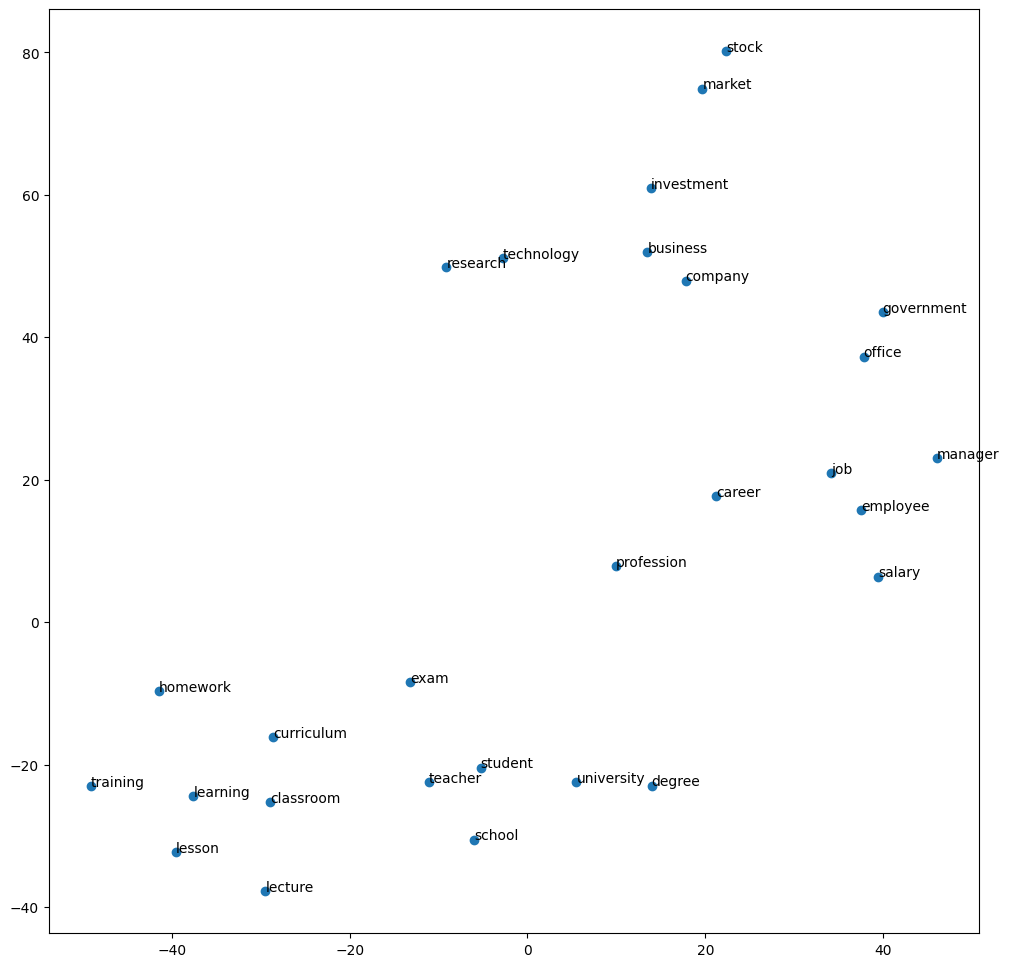
\includegraphics[width=1\textwidth]{images/secAsub6.png}
\caption{Dimensionality reduction and visualization of word embeddings.}
\end{figure}

In the diagram, we can see how words of similar contextual meaning are clustered in the diagram. This happens because the model we've used to retrieve the embeddings from (Glove) was trained on a corpus in which these words were usually found in the same context. From this context, the model created word embedding whose distance is kind of close to each other.

Clear example are the words: "curriculum", "training", "learning", "classroom", "lecture", "lesson", and "homework" all seem to cluster to each other.

We can further verify our statement by pulling the closes word embeddings to one of the words in the cluster, preferrably the one in the center of the cluster - "learning". We should be able to match more words from our list by increasing the topn variable.

%---%

\section*{B. Traditional Text Classification}

\subsection*{1}

The code for the models is located in my notebook named part-B.ipynb

\subsection*{2}

In this scenario, I calculate "Time Cost" as the sum of 3 parts: Vectoriazation, Training and Inference as it's not specified in the assignment. Time details are listed in my notebook: part-B.

\begin{table}[H]
\begin{tabular}{|c|c|c|c|c|}
\hline
\textbf{}      & \textbf{\begin{tabular}[c]{@{}c@{}}ΝΒ\\ (word 1-grams)\end{tabular}} & \textbf{\begin{tabular}[c]{@{}c@{}}NB\\ (char 3-grams)\end{tabular}} & \textbf{\begin{tabular}[c]{@{}c@{}}SVM\\ (word 1-grams)\end{tabular}} & \textbf{\begin{tabular}[c]{@{}c@{}}SVM\\ (char 3-grams)\end{tabular}} \\ \hline
Accuracy       & 0.89                                                                 & 0.85                                                                 & 0.91                                                                  & 0.90                                                                  \\ \hline
Dimensionality & 60734                                                                & 27301                                                                & 60734                                                                 & 27301                                                                 \\ \hline
Time cost      & 1.77                                                                 & 7.26                                                                 & 4.36                                                                  & 11.45                                                                 \\ \hline
\end{tabular}
\end{table}


%---%

\subsection*{3}

I found all models to missclassify text in the following categories:

\begin{lstlisting}
192 missed in category: 1
64 missed in category: 2
260 missed in category: 3
240 missed in category: 4
\end{lstlisting}

One example of such text is the following:

\begin{lstlisting}
AP - It's barely dawn when Mike Fitzpatrick starts his shift with a
blur of colorful maps, figures and endless charts, but already he
knows what the day will bring. Lightning will strike in places he
expects. Winds will pick up, moist places will dry and flames will
roar.

Actual category: 4
Predicted cat: 2

\end{lstlisting}

%---%

\section*{Γ. Text Classification with RNNs}

I updated the training function to track the training times of the models.

\begin{lstlisting}[language=Python]
def TrainModel(model, loss_fn, optimizer, train_loader, epochs):
    training_times = []
    for i in range(1, epochs + 1):
        epoch_start_time = time()
        model.train()
        print('Epoch:', i)
        losses = []

        for X, Y in tqdm(train_loader):
            logits = model(X)
            loss = loss_fn(logits, Y)
            losses.append(loss.item())

            optimizer.zero_grad()
            loss.backward()
            optimizer.step()

        epoch_end_time = time()
        epoch_time_delta = epoch_end_time - epoch_start_time
        training_times.append(epoch_time_delta)
\end{lstlisting}

I created new classes for each requested model as follows. I used \lstinline{pytorch.nn.module} to create the respective model layers and parametrized them with the option for bidirectionality and model \lstinline{input/output} sizes. Where bidirectional models were used, I assumed the \lstinline{Linear} layer to take twice the input of the \lstinline{hidden_dim}. Where 2 linear layers were used, I assumed the output of the first to be equal to \lstinline{hidden_dim} and the input of the next to be twice as large. I used \lstinline{ReLU} as a step function between linear layers.

\textbf{1Bi-RNN}
\begin{lstlisting}[language=Python]
class BidirectionalRNNOneLayer(nn.Module):
    def __init__(self, input_dim, embedding_dim, hidden_dim, output_dim, pad_idx):
        super().__init__()
        self.embedding_layer = nn.Embedding(
            num_embeddings=input_dim, # Dictionary size
            embedding_dim=embedding_dim, # Embedding output
            padding_idx=pad_idx
        )
        self.rnn = nn.RNN(
            input_size=embedding_dim, # RNN input from embeding layer
            hidden_size=hidden_dim,
            batch_first=True,
            bidirectional=True
        )
        self.linear = nn.Linear(2*hidden_dim, output_dim)

    def forward(self, X_batch):
        embeddings = self.embedding_layer(X_batch)
        output, hidden = self.rnn(embeddings)
        # print(output.shape)
        logits = self.linear(output[:, -1, :])   # raw logits
        return logits
\end{lstlisting}

\textbf{2Bi-RNN}
\begin{lstlisting}[language=Python]
class BidirectionalRNNTwoLayer(nn.Module):
    def __init__(self, input_dim, embedding_dim, hidden_dim, output_dim, pad_idx):
        super().__init__()
        self.embedding_layer = nn.Embedding(
            num_embeddings=input_dim, # Dictionary size
            embedding_dim=embedding_dim, # Embedding output
            padding_idx=pad_idx
        )
        self.rnn = nn.RNN(
            input_size=embedding_dim, # RNN input from embeding layer
            hidden_size=hidden_dim,
            batch_first=True,
            bidirectional=True
        )
        self.linear1 = nn.Linear(2*hidden_dim, hidden_dim)
        self.relu = nn.ReLU()
        self.linear2 = nn.Linear(hidden_dim, output_dim)


    def forward(self, X_batch):
        embeddings = self.embedding_layer(X_batch)
        output, hidden = self.rnn(embeddings)
        # print(output.shape)
        logits = self.linear2(self.relu(self.linear1(output[:, -1, :])))   # raw logits
        return logits
\end{lstlisting}

\textbf{1LSTM}
\begin{lstlisting}[language=Python]
class LSTMOneLayer(nn.Module):
    def __init__(self, input_dim, embedding_dim, hidden_dim, output_dim, pad_idx):
        super().__init__()
        self.embedding_layer = nn.Embedding(
            num_embeddings=input_dim, # Dictionary size
            embedding_dim=embedding_dim, # Embedding output
            padding_idx=pad_idx
        )
        self.lstm = nn.modules.rnn.LSTM(
            input_size=embedding_dim, # RNN input from embeding layer
            hidden_size=hidden_dim,
            batch_first=True,
            bidirectional=False
        )
        self.linear1 = nn.modules.Linear(hidden_dim, output_dim)


    def forward(self, X_batch):
        embeddings = self.embedding_layer(X_batch)
        output, hidden = self.lstm(embeddings)
        # print(output.shape)
        logits = self.linear1(output[:, -1, :])   # raw logits
        return logits
\end{lstlisting}

\textbf{1Bi-LSTM}
\begin{lstlisting}[language=Python]
class BidirectionalLSTMOneLayer(nn.Module):
    def __init__(self, input_dim, embedding_dim, hidden_dim, output_dim, pad_idx):
        super().__init__()
        self.embedding_layer = nn.Embedding(
            num_embeddings=input_dim, # Dictionary size
            embedding_dim=embedding_dim, # Embedding output
            padding_idx=pad_idx
        )
        self.lstm = nn.modules.rnn.LSTM(
            input_size=embedding_dim, # RNN input from embeding layer
            hidden_size=hidden_dim,
            batch_first=True,
            bidirectional=True
        )
        self.linear1 = nn.modules.Linear(2*hidden_dim, output_dim)


    def forward(self, X_batch):
        embeddings = self.embedding_layer(X_batch)
        output, hidden = self.lstm(embeddings)
        # print(output.shape)
        logits = self.linear1(output[:, -1, :])   # raw logits
        return logits
\end{lstlisting}

\textbf{2Bi-LSTM}
\begin{lstlisting}[language=Python]
class BidirectionalLSTMTwoLayer(nn.Module):
    def __init__(self, input_dim, embedding_dim, hidden_dim, output_dim, pad_idx):
        super().__init__()
        self.embedding_layer = nn.Embedding(
            num_embeddings=input_dim, # Dictionary size
            embedding_dim=embedding_dim, # Embedding output
            padding_idx=pad_idx
        )
        self.lstm = nn.modules.rnn.LSTM(
            input_size=embedding_dim, # RNN input from embeding layer
            hidden_size=hidden_dim,
            batch_first=True,
            bidirectional=True
        )
        self.linear1 = nn.modules.Linear(2*hidden_dim, hidden_dim)
        self.relu = nn.ReLU()
        self.linear2 = nn.modules.Linear(hidden_dim, output_dim)

    def forward(self, X_batch):
        embeddings = self.embedding_layer(X_batch)
        output, hidden = self.lstm(embeddings)
        # print(output.shape)
        logits = self.linear2(self.relu(self.linear1(output[:, -1, :])))   # raw logits
        return logits
\end{lstlisting}

I updated the main loop which builds and trains the model to reflect the requested. Here, I only present one snapshot of that loop which is adjusted to use the respective model.


\begin{lstlisting}
training_times = []
accuracies = []

for i in range(3):
  classifier = BidirectionalRNNOneLayer(len(itos), EMBEDDING_DIM, HIDDEN_DIM, len(target_classes), PAD_IDX).to(device)
  loss_fn = nn.CrossEntropyLoss()
  optimizer = torch.optim.Adam(classifier.parameters(), lr=LEARNING_RATE)
  print('\nModel:')
  print(classifier)
  print('Total parameters:', count_parameters(classifier))
  print('\n')

  print(f"Iteration: {i}")
  times = TrainModel(classifier, loss_fn, optimizer, train_loader, EPOCHS)
  training_times.append(times)
  _, Y_actual, Y_preds = EvaluateModel(classifier, loss_fn, test_loader)

  accuracy = accuracy_score(Y_actual, Y_preds)
  accuracies.append(accuracy)

print(f"Mean Accuracy: {np.mean(accuracies):.3f}")
print(f"Std. Accuracy: {np.std(accuracies):.3f}")
print(f"Mean Time: {np.mean(training_times):.3f}")
\end{lstlisting}

%---%

\subsection*{1}

\begin{table}[H]
\begin{tabular}{|l|c|c|c|c|c|c|}
\hline
\multicolumn{1}{|c|}{\textbf{}} & \textbf{1RNN} & \textbf{1Bi-RNN} & \textbf{2Bi-RNN} & \textbf{1LSTM} & \textbf{1Bi-LSTM} & \textbf{2Bi-LSTM} \\ \hline
\textbf{Mean Accuracy}          & 0.881         & 0.885            & 0.876            & 0.883          & 0.882             & 0.882             \\ \hline
\textbf{Std. Accuracy}          & 0.001         & 0.001            & 0.002            & 0.004          & 0.002             & 0.002             \\ \hline
\textbf{Parameters}             & 1974384       & 1985264          & 1993264          & 2006256        & 2049008           & 2057008           \\ \hline
\textbf{Time cost}              & 3.98          & 3.717            & 3.746            & 3.796          & 4.184             & 4.124             \\ \hline
\end{tabular}
\end{table}

All network architectures present a consistency across evaluation metrics. It's natural for LSTM type networks to have a slightly higher training times and an increased number of parameters. Moreover, I noticed a difference of $0.1$ in the final training loss between RNN and LSTM type models.

%---%

\subsection*{2}

With the average training time for the 1RNN being at 11.277 sec. and 25.813 sec. for 1LSTM, there's a signification time reduction offered by the accelerator.

%---%

\subsection*{3}


\begin{figure}[H]
\centering
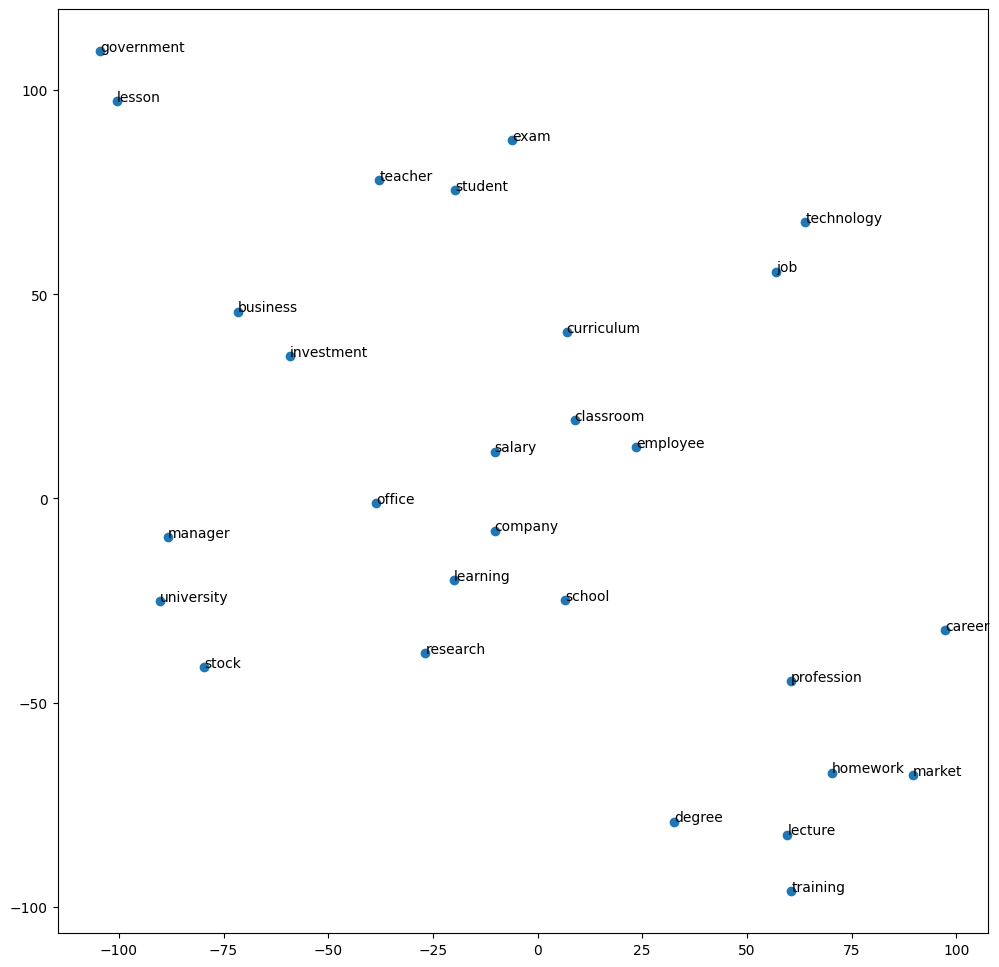
\includegraphics[width=1\textwidth]{images/secCsub3.png}
\end{figure}

As expected, the pretrained word embeddings from \lstinline{word2vec} and \lstinline{GloVe} models show a better coherence than the ones we created using the limited dataset (AG news).

%---%
\subsection*{4}

\begin{table}[H]
\begin{tabular}{|l|c|c|c|c|c|c|}
\hline
\multicolumn{1}{|c|}{\textbf{}} & \textbf{1RNN} & \textbf{1Bi-RNN} & \textbf{2Bi-RNN} & \textbf{1LSTM} & \textbf{1Bi-LSTM} & \textbf{2Bi-LSTM} \\ \hline
\textbf{Mean Accuracy}          & 0.877         & 0.713            & 0.621            & 0.902          & 0.9               & 0.882             \\ \hline
\textbf{Std. Accuracy}          & 0.007         & 0.224            & 0.173            & 0.000          & 0.004             & 0                 \\ \hline
\textbf{Parameters}             & 1974384       & 1985264          & 1993264          & 2006256        & 2049008           & 2057008           \\ \hline
\textbf{Time cost}              & 4.097         & 4.073            & 4.123            & 4.291          & 4.524             & 17.08             \\ \hline
\end{tabular}
\end{table}

We can see how RNNs struggle to classify sentences in the training dataset, thus their accuracy drops. Linear layers don't maintain any word context and their addition reduces the accuracy even further. This is expected considering that RNNs struggle tracking word context as sentences grow past 20 words per sentence.

On the other hand, LSTM networks are able to maintain high accuracies on these new, larger, sentences which is attributed to their memory mechanism which allows them to maintain word context in large sentences.

Furthermore, we can see a slight increase in training times which is attributed to the doubling of the sentence size - more processing is required.

%---%

\subsection*{5}

The main changes to the code were with regards to using the embeddings from \lstinline{GloVe}. Following is a code snippet which shows how I extracted the embeddings and created a 2D tensor and used it as the first layer in the model. It's important to note that classmethod \lstinline{.from_pretrained()} has \lstinline{freeze=True} by default - here we explicitly set it to \lstinline{False}.

\begin{lstlisting}[language=Python]

# Download the embeddings
import os
import zipfile
with zipfile.ZipFile('/tmp/glove.6B.zip', 'r') as zip_ref:
    zip_ref.extractall('/tmp/glove')

# Create 2D tensor
word_embeddings = []
with open('/tmp/glove/glove.6B.100d.txt', "r") as f:
  for line in f.readlines():
    np_array = np.array(line.split()[1:])
    word_embeddings.append( np_array.astype("float32") )


# Load tensor in the model
class Model1Bi_RNN(nn.Module):
    def __init__(self, word_embeddings_tensor, dic_size, embedding_dim, hidden_dim, output_dim, pad_idx):
        super().__init__()
        self.embedding_layer = nn.Embedding(
            num_embeddings=dic_size, # Dictionary size
            embedding_dim=embedding_dim, # Embedding output
            padding_idx=pad_idx
        ).from_pretrained(word_embeddings_tensor, freeze=False)

        self.rnn = nn.RNN(
            input_size=embedding_dim, # RNN input from embeding layer
            hidden_size=hidden_dim,
            batch_first=True,
            bidirectional=True
        )
        self.linear = nn.Linear(2*hidden_dim, output_dim)

    def forward(self, X_batch):
        embeddings = self.embedding_layer(X_batch)
        output, hidden = self.rnn(embeddings)
        logits = self.linear(output[:, -1, :])   # raw logits
        return logits
\end{lstlisting}

I used the same results extraction function, defined above. Details of the implementations of the rest of the neural networks are provided in the notebook.

\begin{table}[H]
\begin{tabular}{|l|c|c|c|c|c|c|}
\hline
\multicolumn{1}{|c|}{\textbf{}} & \textbf{1RNN} & \textbf{1Bi-RNN} & \textbf{2Bi-RNN} & \textbf{1LSTM} & \textbf{1Bi-LSTM} & \textbf{2Bi-LSTM} \\ \hline
\textbf{Mean Accuracy}          & 0.883         & 0.880            & 0.881            & 0.886          & 0.888             & 0.888             \\ \hline
\textbf{Std. Accuracy}          & 0.003         & 0.007            & 0.003            & 0.004          & 0.000             & 0.004             \\ \hline
\textbf{Parameters}             & 40010884      & 40021764         & 40029764         & 40042756       & 40085508          & 40093508          \\ \hline
\textbf{Time cost}              & 4.398         & 3.841            & 3.888            & 3.963          & 4.245             & 4.218             \\ \hline
\end{tabular}
\end{table}

The performance remains strongly consistent ($~88\%$) across model architectures. The dictionary of the word embeddings imprints well the one from our dataset. It's important to note how the parameters of the respective neural networks, in this task, have increased tens of millions compared to the ones from task 1. This is expected, since the embedding layers now has the size of the dictionary of the pre-trained embeddings, $400,000 words * 100 dimensions = 40,000,000 parameters$.

%---%

\subsection*{6}

The only changed implemented in the neural net architectures was to set the \lstinline{freeze} parameter to \lstinline{True} - the rest remained the same.

\begin{table}[H]
\begin{tabular}{|l|c|c|c|c|c|c|}
\hline
\multicolumn{1}{|c|}{\textbf{}} & \textbf{1RNN} & \textbf{1Bi-RNN} & \textbf{2Bi-RNN} & \textbf{1LSTM} & \textbf{1Bi-LSTM} & \textbf{2Bi-LSTM} \\ \hline
\textbf{Mean Accuracy}          & 0.703         & 0.711            & 0.698            & 0.820          & 0.815             & 0.816             \\ \hline
\textbf{Std. Accuracy}          & 0.015         & 0.010            & 0.017            & 0.003          & 0.007             & 0.009             \\ \hline
\textbf{Parameters}             & 10884         & 21764            & 29764            & 42756          & 85508             & 93508             \\ \hline
\textbf{Time cost}              & 4.068         & 4.928            & 5.356            & 5.119          & 4.667             & 4.564             \\ \hline
\end{tabular}
\end{table}

In this case, the performance remains bellow the one from the previous task. The training process does not train the embeddings (frozen) and does not adjust them to the dictionary of our dataset well. Training only the weights of the neural networks, results in poorer performance.

By setting \lstinline{freeze=True}, we also set \lstinline{embedding.weight.requires_grad = False} which prevents the embeddings from adjusting during gradient descent. \lstinline{PyTorch} only lists the parameters which are trained by gradient descent, which in this case, are only the weights of the neural networks (excluding embeddings).

%---%

\subsection*{7}

Following are the most important code snippets I implemented for the expriements using the IMDB dataset.

\begin{lstlisting}[language=Python]
# Download dataset
path = kagglehub.dataset_download("lakshmi25npathi/imdb-dataset-of-50k-movie-reviews", output_dir="/content/data2")

# Read dataset
dataset = pd.read_csv(f"{path}/IMDB Dataset.csv")
X = dataset["review"]
y = dataset["sentiment"]

# Convert class to int
y = y.astype("category").cat.codes

# Split
X_train, X_test, y_train, y_test = train_test_split(X, y, test_size=0.20)

# Build datasets
train_dataset = [
    (sentiment, review)
    for sentiment, review in zip(y_train, X_train)
]
test_dataset = [
    (sentiment, review)
    for sentiment, review in zip(y_test, X_test)
]
target_classes = ["negative", "positive"]

# Fix collate function
def collate_batch(batch):
    Y, X = list(zip(*batch))
    Y = torch.tensor(Y, dtype=torch.long)

    X = [numericalize(text) for text in X]
    X = [
        tokens + [PAD_IDX] * (MAX_WORDS - len(tokens))
        if len(tokens) < MAX_WORDS else tokens[:MAX_WORDS]
        for tokens in X
    ]
\end{lstlisting}

The code for the neural network architectures remained pretty much the same. Detailed implementations are provided in the notebook \lstinline{part-C.ipynb}. I trained all the neural networks, in this task, on a CPU.

\begin{table}[H]
\begin{tabular}{|l|c|c|c|c|c|c|}
\hline
\multicolumn{1}{|c|}{\textbf{}} & \textbf{1RNN} & \textbf{1Bi-RNN} & \textbf{2Bi-RNN} & \textbf{1LSTM} & \textbf{1Bi-LSTM} & \textbf{2Bi-LSTM} \\ \hline
\textbf{Mean Accuracy}          & 0.721         & 0.717            & 0.709            & 0.715          & 0.715             & 0.712             \\ \hline
\textbf{Std. Accuracy}          & 0.005         & 0.004            & 0.005            & 0.004          & 0.005             & 0.005             \\ \hline
\textbf{Parameters}             & 2560554       & 2571306          & 2579434          & 2592426        & 2635050           & 2635050           \\ \hline
\textbf{Time cost}              & 11.724        & 14.980           & 13.107           & 18.216         & 29.737            & 29.698            \\ \hline
\end{tabular}
\end{table}

%---%

\section*{Addendum}

Experimenting on Colab using the GPU, resulted in running out of free tokens, so I had to run some of the experiments on the CPU.

% \bibliographystyle{plain}
%
% {\small
% \bibliography{refs}}

\clearpage % Start Bibliography on a new page
\nocite{*}
\phantomsection
\addcontentsline{toc}{chapter}{Bibliography} % <--- ADDS the entry to the TOC
\begingroup % Start a group to localize changes (like font size)
\footnotesize % Apply the desired font size
\bibliographystyle{plain}
\bibliography{refs}
\endgroup % End the local group

\end{document}
